\lab{Algorithms}{Statistical Distributions}{Statistical Distributions}
\label{lab:distributions}
\objective{This section will review the most common distributions and thus assumes prior exposure to basic terms and concepts.}

\section*{Discrete Distributions}
\emph{Discrete distributions} are distributions whose support is finite or countable at most. 
The \emph{support} of a distribution refers to the points in $\mathbb{R}$ that have non-zero probability. 
In other words, discrete distributions are a collection of point masses. 

\begin{table*}[h]
\centering
\begin{tabular}{|c|c|c|c|}
	\hline
 & Uniform &  Binomial & Poisson \\
\hline 
\hline
Support&$x \in \{a,\dots,b\}$&$x \in \{0,\dots,n\}$&$x \in \{0,1,2,\dots\}$\\ \hline
PMF&$\frac{1}{b-a+1}$&$\dbinom{n}{x}p^x(1-p)^{n-x}$&$\frac{e^\lambda \lambda^x}{x!}$\\ \hline
Parameters&$b>a$, $a,b \in \mathbb{Z}$&$n \in \mathbb{N}$, $p \in [0,1]$& $\lambda>0$\\ \hline
Mean $E(X)$&$\frac{a+b}{2}$&$np$& $\lambda$\\ \hline
Variance&&$np(1-p)$& $\lambda$\\ \hline
Description& 
\parbox{1in}{models a single occurrence of one of several events of equal probability} & \parbox{1in}{models $n$ events with binary outcomes, where $p$ is the probability of a success ($x=1$). Note, when $n=1$, this is referred to as the Bernoulli distribution, or a Bernoulli trial.}&\parbox{1in}{models the number of events that occur in a given time period, given rate $\lambda$}\\
\hline
\end{tabular}
\end{table*}

\section*{Continuous Distributions}
\emph{Continuous distributions} are distributions whose support is uncountable, i.e. some subset of $\mathbb{R}$. 
\begin{table*}[h]
\centering
\begin{tabular}{|c|c|c|c|}
	\hline
 & Normal& Gamma&Beta\\ \hline \hline
Support &$x \in \mathbb{R}$ & $x>0$ &$x \in [0,1]$\\  \hline
PDF & $\frac{1}{\sqrt{2\pi \sigma^2}} e^{-\frac{1}{2\sigma^2}(x-\mu)^2}$ & $\frac{\beta^\alpha}{\Gamma(\alpha)} x^{\alpha -1} e^{-\beta x}$ &$\frac{\Gamma(\alpha+\beta)}{\Gamma(\alpha)\Gamma(\beta)} x^{\alpha-1} (1-x)^{\beta-1}$\\  \hline
Parameters & $\mu \in \mathbb{R}$, $\sigma^2 > 0$ & $\alpha,\beta>0$ &$\alpha,\beta>0$\\  \hline
Mean &  $\mu$& $\frac{\alpha}{\beta}$ &$\frac{\alpha}{\alpha + \beta}$\\  \hline
Variance &$\sigma^2$& $\frac{\alpha}{\beta^2}$&$\frac{\alpha \beta}{(\alpha + \beta)^2(\alpha + \beta +1)}$\\ \hline
Description&The bell curve&\parbox{1in}{When $\alpha=1$, this is called the exponential distribution. $\alpha$ is called the shape, $\beta$ is called the rate.}&\parbox{1in}{models probabilities or proportions. When $\alpha = \beta =1$, this is called the continuous uniform distribution}\\
\hline
\end{tabular}
\end{table*}

\section*{Normal Distribution}
The SAT is a standardized test common for college admissions in the United States. 
It is comprised of three sections, critical reading, writing and mathematics. 
Each section is graded out of 800 possible points, with a minimum score of 200.
Each section is intended to have a mean score of 500 with a standard deviation of 100.  
The distribution of SAT section scores is well approximated by the normal distribution 
(though these scores are discrete and to the nearest 10, i.e. $\mbox{score} \in \{200,210,220,\dots,790,800\}$, we are only approximating it). 
\begin{figure}[h]
\includegraphics[width=\textwidth]{normaldist.pdf}
\end{figure}

The scores of the three sections are added together to produce the test score. 
Thus the test in aggregate has 2400 possible points and a minimum score of 600.  
As each of the three sections has a mean score of 500 and a standard deviation of 100, it seems logical that the test score would also has a normal distribution, 
but with mean of 1500 points and a standard deviation of 300 points. 
But is that true? One method of evaluating this is to simulate the test scores and then find the mean and standard deviation of our simulated data. 
NumPy provides a tool to generate random data from the normal distribution, numpy.random.normal.

\begin{problem}
Generate 10,000 random test scores by adding together three vectors of 10,000 random draws from the $N(\mu=500,\sigma=100)$ distribution. 
Find the mean and standard deviation of the 10,000 test scores. 
Are they close to 1500 and 300, respectively? 
Also, make a histogram of the test scores to visually inspect for whether or not the test scores are also normally distributed.
\label{prob:randomTests}
\end{problem}

\begin{figure}[h]
\includegraphics[width=\textwidth]{scorehist.pdf}
\caption{Histogram of the simulated test scores.}
\end{figure}
In the plot above, we see that the the 10,000 randomly generated test scores appear to be fairly bell-shaped, i.e. normally distributed. 
The mean of these test scores should, in fact, be about 1500. 
However, the standard deviation is not $3(100) = 300$, but around 173.2, or $\sqrt{3*100^2}=\sqrt{3}(100) \approx 173.205081$. 
This is because, for independent normal random variables $X_1 \sim N(\mu_1,\sigma^2_1), X_2 \sim N(\mu_2,\sigma^2_2),X_3 \sim N(\mu_3,\sigma^2_3),$
\[ (X_1 +X_2 +X_3) \sim N(\mu_1+\mu_2+\mu_3, \sigma^2_1+\sigma^2_2+\sigma^2_3). \]
Said succinctly, the mean of the sum is the sum of the means, and the variance of the sum is the sum of the variances. 
But as the standard deviation is the square root of the variance, this same idea doesn't work. 
Yet we do see that the standard deviation of the sum is the square root of the sum of the variances (the new variance):
\[ \sqrt{100^2+100^2+100^2} = \sqrt{30000} \approx 173.205081 \]

\section*{Multivariate Normal Distribution}
Note that in problem \ref{prob:randomTests}, we assumed that the scores of all three tests were independent. 
This should seem like an unreasonable assumption, because we expect there to be at least a little correlation in the test scores, 
i.e. a student with a high reading score is more likely to score high on the other sections compared to a student with a low reading score. 
To employ correlations in these draws, we turn to the multivariate normal distribution. 
\begin{table*}[h]
\centering
\begin{tabular}{|c|c|}
\hline
&Multivariate Normal distribution  \\ \hline \hline
Support &$\mathbf{x} \in \mathbb{R}^k$ \\ \hline
PDF & $(2\pi)^{-k/2}|\Sigma|^{-1/2}e^{-\frac{1}{2}(\mathbf{x} - \mathbf\mathbf{\mu})^T \Sigma^{-1} (\mathbf{x}-\mathbf{\mu})}$ \\ \hline
 Parameters&$\mathbf{\mu}\in \mathbb{R}^k, \Sigma \in \mathbb{R}^{k\times k}$ \\ \hline
\end{tabular}
\end{table*}
Note that there is no mean and variance included above. 
Similar to the normal distribution, they are simply $\mu$ and $\Sigma$ respectively. Also note that for $k=1$, this is the normal distribution.  
Furthermore, this distribution can be viewed as having $k$ components, each of which is normally distributed. 
Thus, $\mathbf{\mu}$ is a vector of the means of each of these normal distributions. 
Similarly, the diagonal of the matrix $\Sigma$ are the variances of the $k$ components. 
The off-diagonal elements of $\Sigma$ are covariances, or in other words, $\Sigma_{i,j} = Cov(x_i,x_j) = \sigma_i \sigma_j \rho_{ij}$, where $\rho_{ij}$ is the correlation between $x_i$ and $x_j$. 
Hence, for $i=j$, $\Sigma_{i,j} = \sigma^2_i$ as the correlation between an object and itself is 1. 

Returning to our SAT example, we can use the multivariate normal distribution with $k=3$. 
Because each distribution of section scores has a mean of 500 and a variance of 10,000, $\mathbf{\mu} = (500,500,500)$ and $\Sigma_{1,1} = \Sigma_{2,2} = \Sigma_{3,3} = 10,000$. 
Now let's assume the correlation between the reading and writing sections is $.7$, and the others are $.5$. 
This means for $\mathbf{x} = (x_{\text{math}},x_{\text{read}},x_{\text{write}})$
\[ \Sigma =  \begin{bmatrix*}
10000 & 5000 & 5000 \\
5000 & 10000 & 7000 \\
5000 & 7000 & 10000 \end{bmatrix*} \]  

\begin{problem}
Using the above $\mathbf{\mu}$ and $\Sigma$, generate 10,000 random test scores by adding together the vectors created by 10,000 random draws from the 
\li{numpy.random.multivariate_normal} function. 
Find the mean and standard deviation of the 10,000 test scores and make a histogram of the test scores to visually 
inspect for whether or not the test scores are also normally distributed. 
Which of the models discussed appears to be more appropriate?
\end{problem}

Note that the mean of the generated scores should be around 1500 and the standard deviation $\sqrt{64000} \approx 253$. 
Note that 64,000 is the sum of all elements in $\Sigma$, however the explanation is beyond the scope of this lab. 
\begin{figure}[h]
\includegraphics[width=\textwidth]{scorehist-mvn.pdf}
\caption{Histogram of the simulated test scores, generated via the multivariate normal distribution.}
\end{figure}


\section*{Central Limit Theorem}
The Central Limit Theorem, simply stated, says that for independently and identically distributed random variables, $X_i$ , $i = 1, \dots, n$, as $n \rightarrow \infty$,
\[ 
\frac{1}{n} \sum^n_{i=1} X_i = \bar{x}_n \sim N\left(E(X), \frac{Var(X)}{n}\right)
\]
In other words, for a large enough sample size, the sample mean is approximately normally distributed. 
\begin{figure}[h]
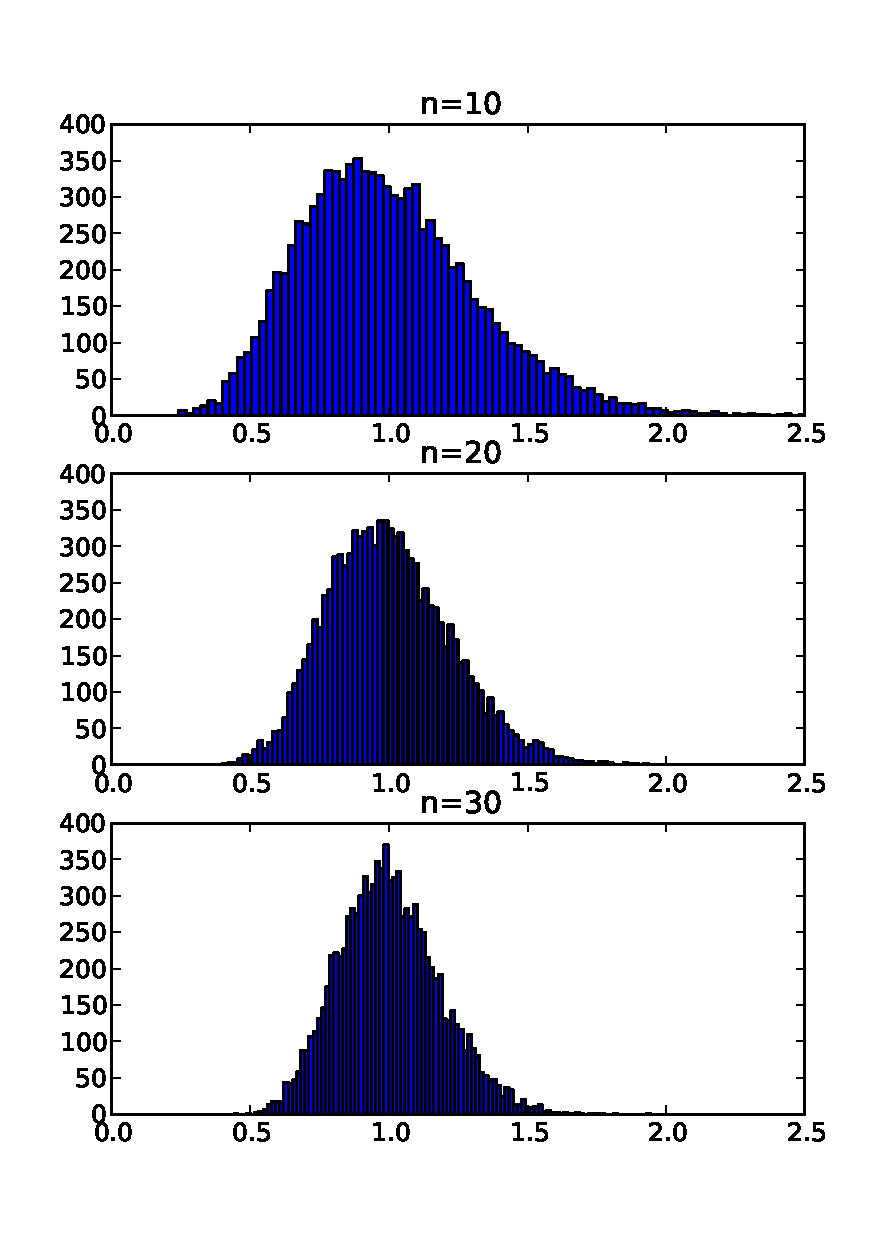
\includegraphics[width=\textwidth]{multiplot.pdf}
\caption{A histogram of the means of 10,000 samples of size 10, 20, and 30 respectively, from the Exponential(1) distribution (same as the Gamma(1,1) distribution). Notice that as $n$ increases, it leaves the shape of the original distribution (exponential) and becomes more and more bell-curve-shaped.}
\label{fig:CLT}
\end{figure}

\begin{problem}
Prove to yourself that the Central Limit Theorem holds for all distributions.  Create plots similar to \ref{fig:CLT} for the Poisson(3), Beta(.1,.1), and the Binomial($n=20$,$p=.8$). Notice how the discrete distributions appear ``more continuous'' as $n$ grows, due to more values being possible. 
\end{problem}
